\documentclass{article}
\usepackage[utf8]{inputenc}
\usepackage{graphicx}

\title{Tugas Besar Laundry}
\author{Rizal Ramadhan }
\date{December 2019}

\begin{document}

\maketitle

\section{Table}

\begin{enumerate}
\item sebelum membuat aplikasi kita harus terlebih dahulu membuat table nya dan table terdiri dari table detergen,petugas,dan transaksi
    
\item table detergen dibuat
    \begin{center}
         \centering
            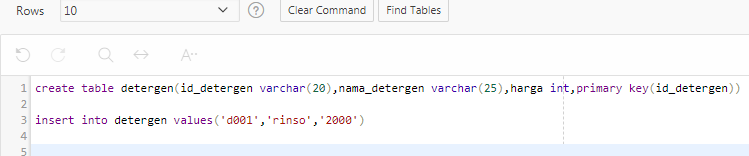
\includegraphics[scale=0.27]{gambar/Capture1.PNG}
        \caption{}
        \label{excel}
    \end{center}

\item table petugas dibuat
    \begin{center}
         \centering
            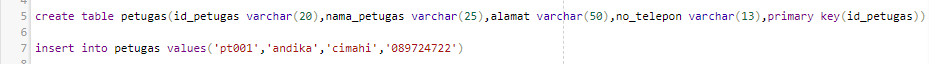
\includegraphics[scale=0.27]{gambar/Capture2.PNG}
        \caption{}
        \label{excel}
    \end{center}
    
\item table transaksi dibuat
    \begin{center}
         \centering
            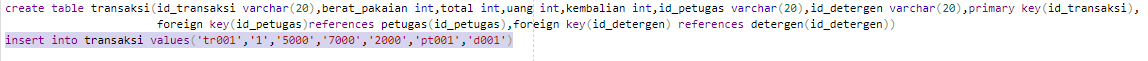
\includegraphics[scale=0.27]{gambar/Capture3.PNG}
        \caption{}
        \label{excel}
    \end{center}
    
\item table yang sudah dibuat 
    \begin{center}
         \centering
            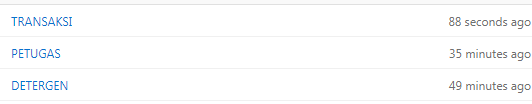
\includegraphics[scale=0.27]{gambar/Capture4.PNG}
        \caption{}
        \label{excel}
    \end{center}
    
\item relasi table nya
    \begin{center}
         \centering
            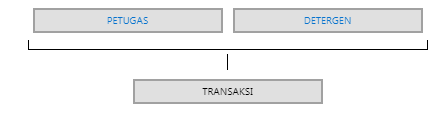
\includegraphics[scale=0.27]{gambar/Capture5.PNG}
        \caption{}
        \label{excel}
    \end{center}
    
\item membuat trigger dimana setiap transaksi yang dilakukan akan ditambah 1000 sebagai bonus
    \begin{center}
         \centering
            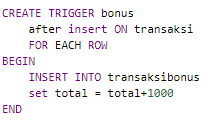
\includegraphics[scale=0.27]{gambar/Capture8.PNG}
        \caption{}
        \label{excel}
    \end{center}
    
\item membuat table view
    \begin{center}
         \centering
            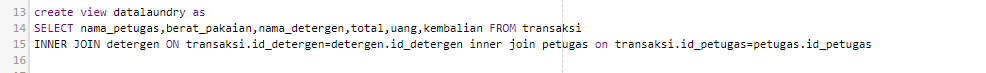
\includegraphics[scale=0.27]{gambar/Capture6.PNG}
        \caption{}
        \label{excel}
    \end{center}

    
\end{enumerate}


\section{pembuatan aplikasi}

\begin{enumerate}
\item disini kita akan membuat aplikasi laundry nya karena database nya sudah selesai dibuat
    
\item masuk ke app builder dan pilih create
    \begin{center}
         \centering
            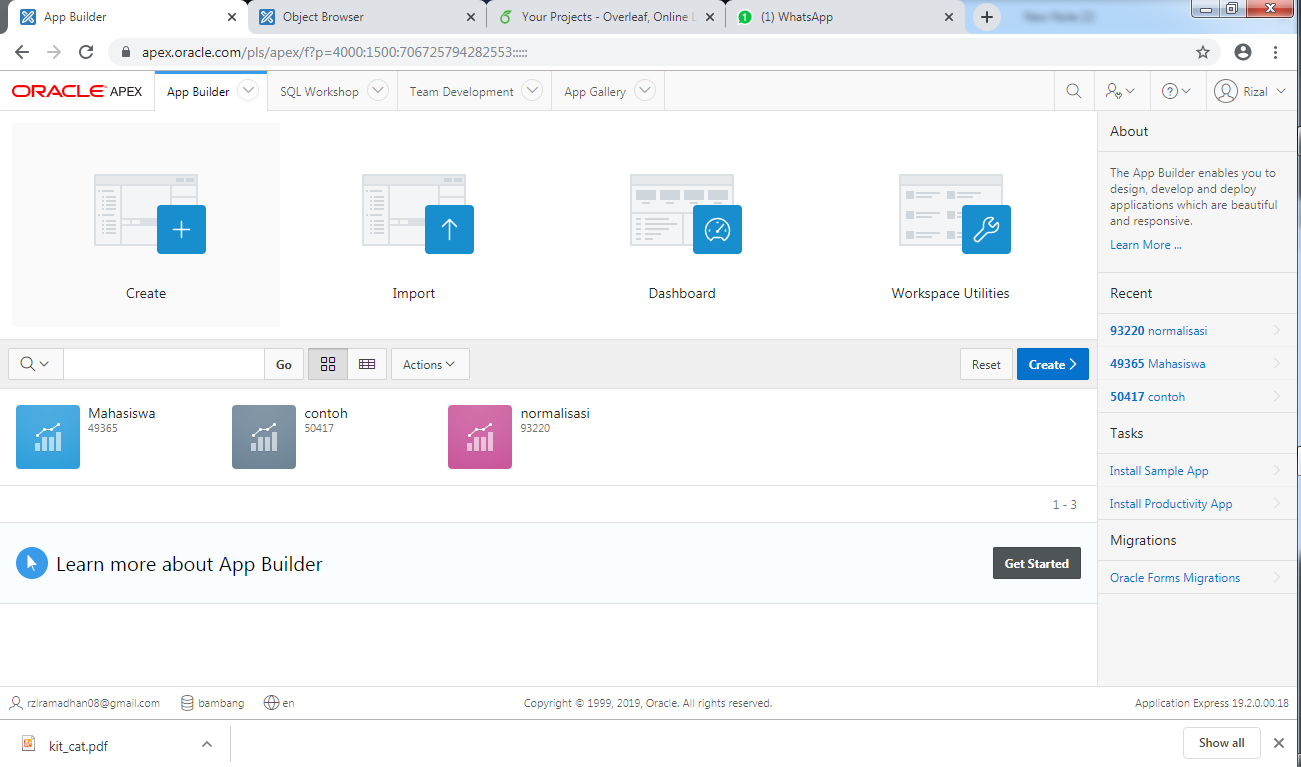
\includegraphics[scale=0.27]{gambar/Capture9.PNG}
        \caption{}
        \label{excel}
    \end{center}

\item setelah itu pilih new application 
    \begin{center}
         \centering
            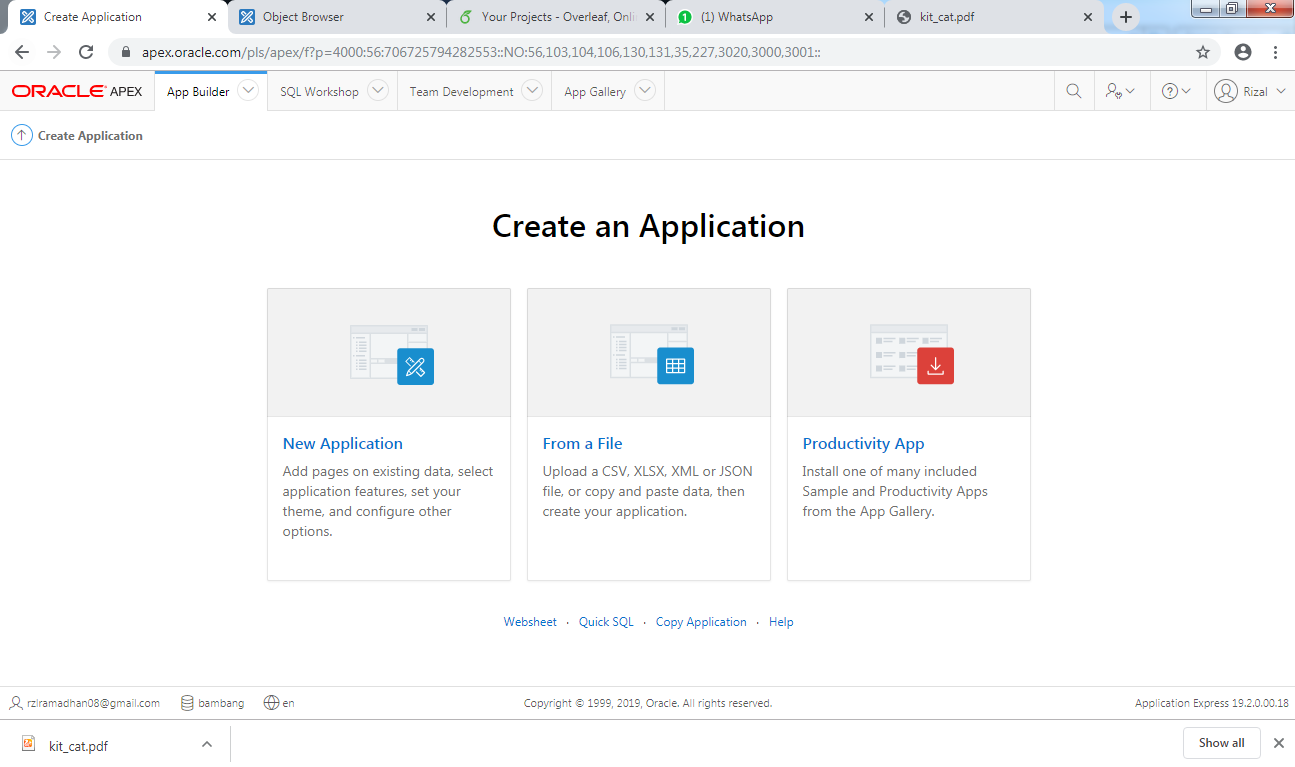
\includegraphics[scale=0.27]{gambar/Capture11.PNG}
        \caption{}
        \label{excel}
    \end{center}    

\item lalu tuliskan aplikasi laundry
    \begin{center}
         \centering
            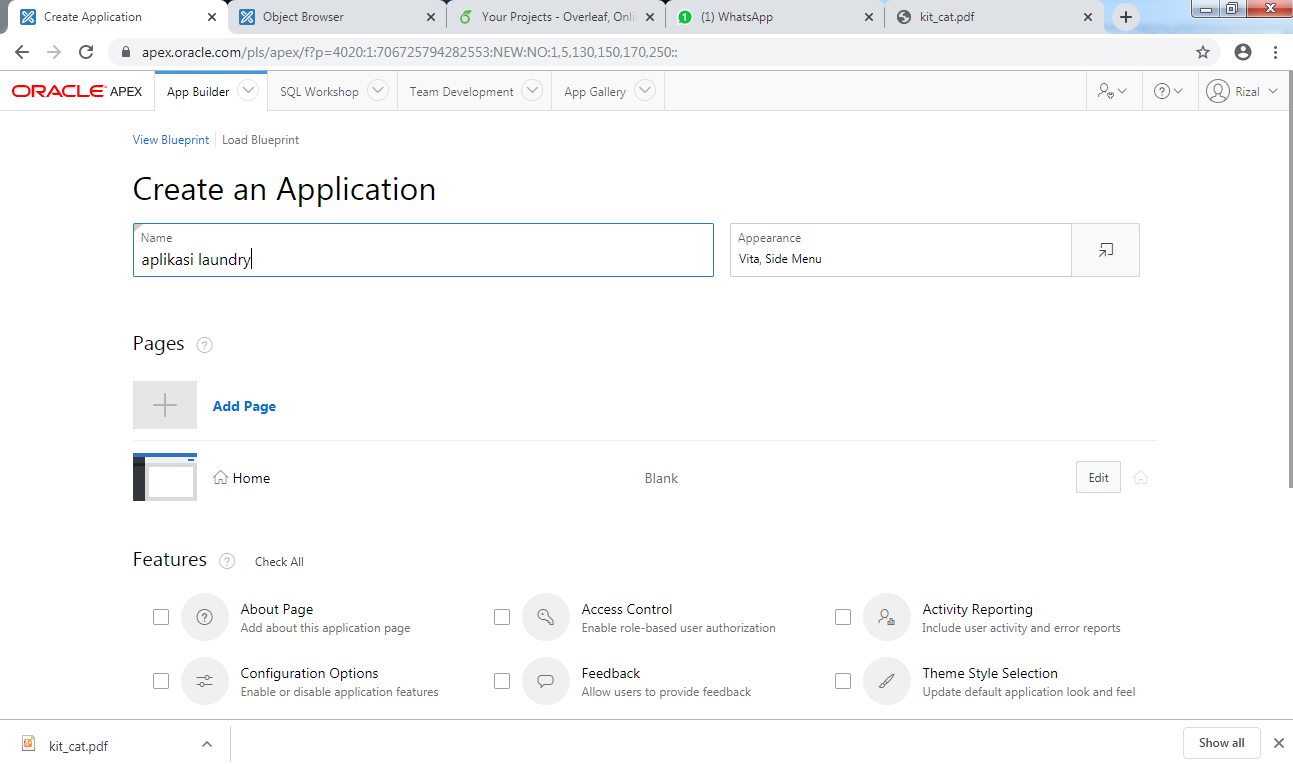
\includegraphics[scale=0.27]{gambar/Capture12.PNG}
        \caption{}
        \label{excel}
    \end{center}   

\item lalu pilih addpage dan pilih page intereactive 
    \begin{center}
         \centering
            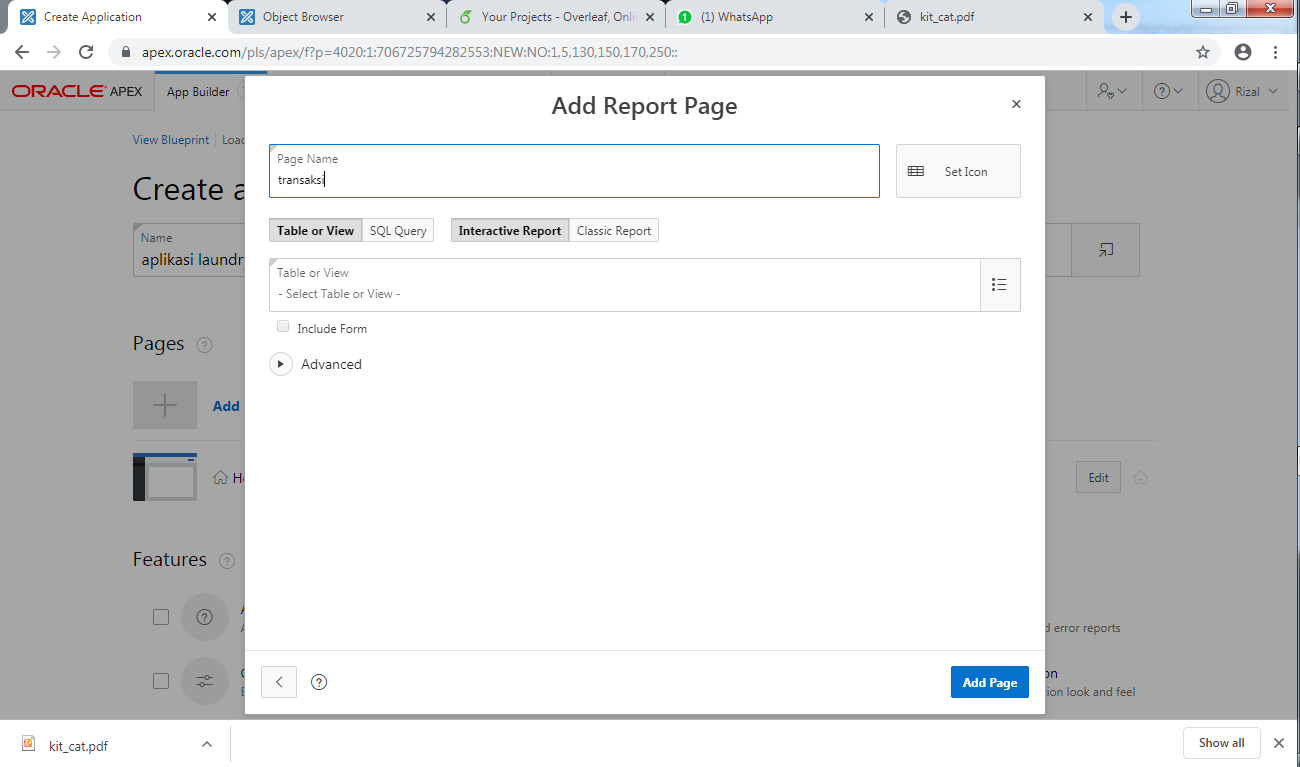
\includegraphics[scale=0.27]{gambar/Capture13.PNG}
        \caption{}
        \label{excel}
    \end{center}  

\item lalu create application
    \begin{center}
         \centering
            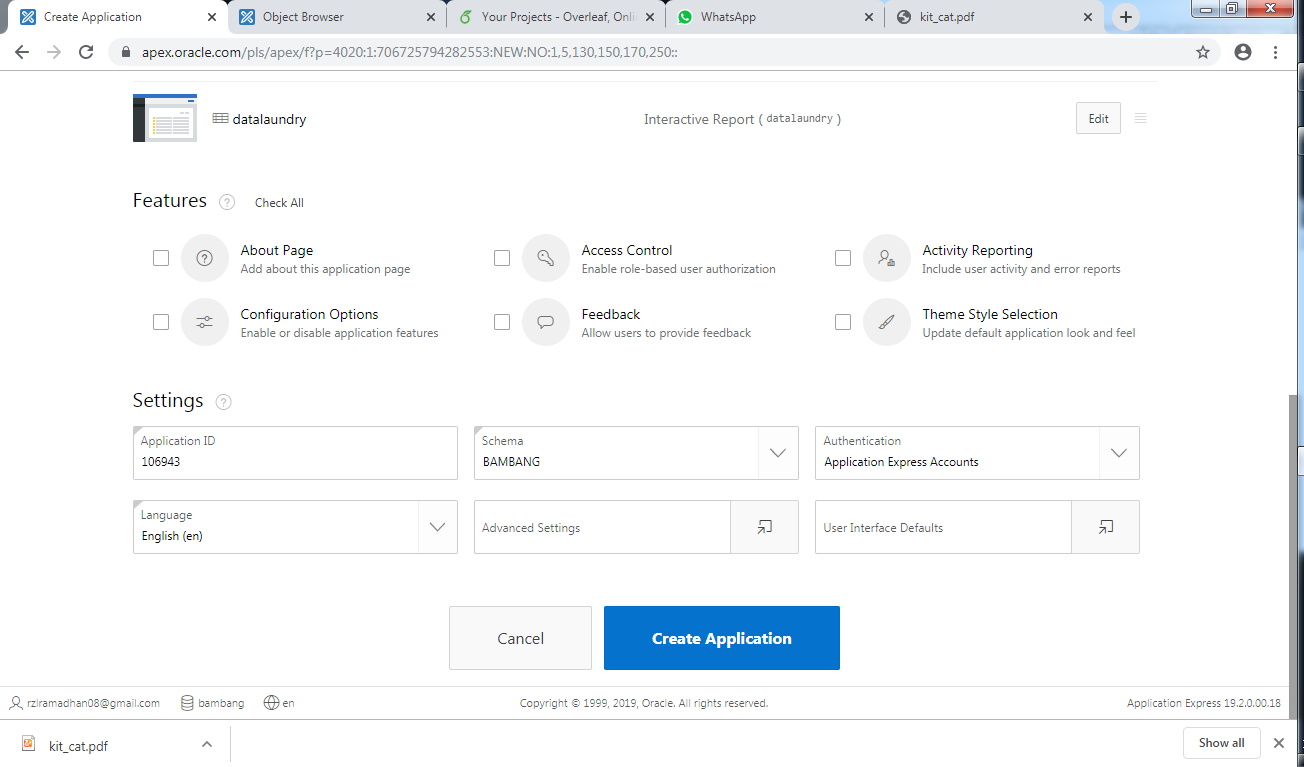
\includegraphics[scale=0.27]{gambar/Capture14.PNG}
        \caption{}
        \label{excel}
    \end{center} 
    
\item lalu setelah itu pilih run application setelah di create 
    \begin{center}
         \centering
            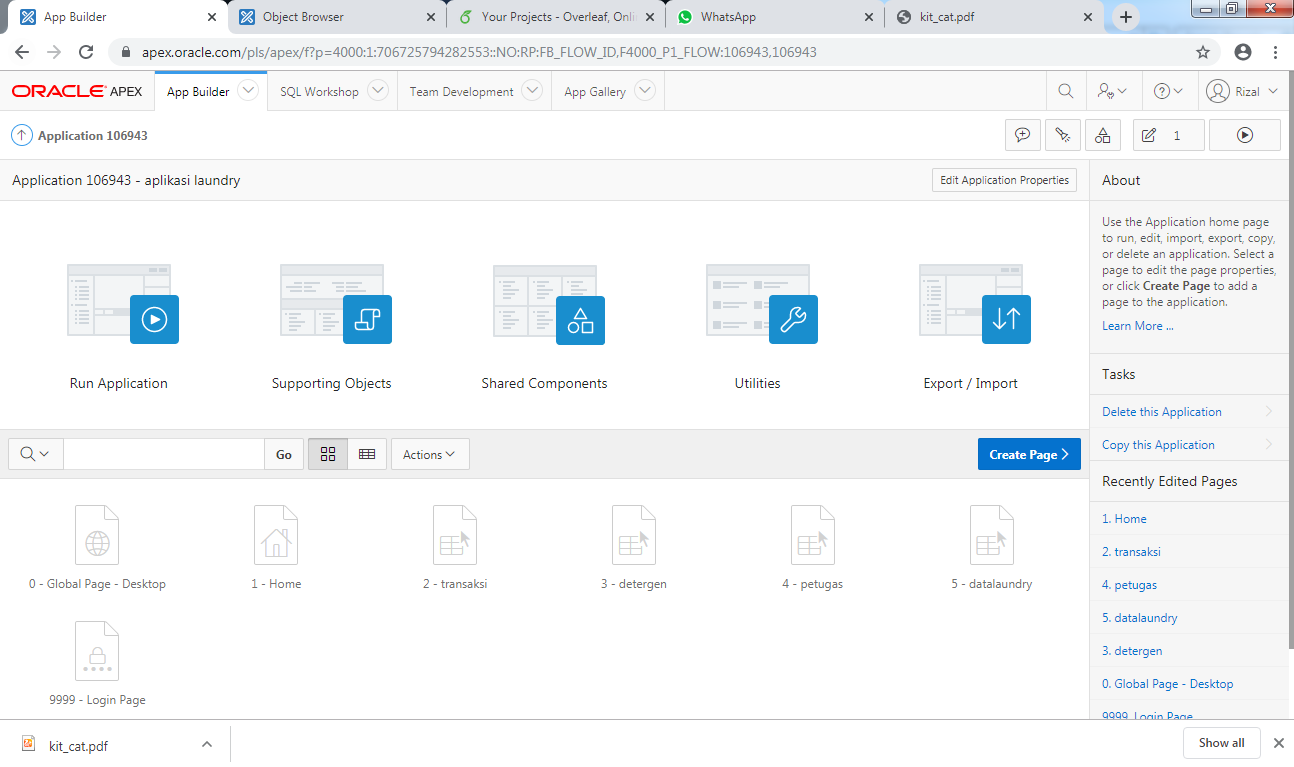
\includegraphics[scale=0.27]{gambar/Capture15.PNG}
        \caption{}
        \label{excel}
    \end{center} 
    
\item lalu masukan username dan password nya nanti akan saya sediakan di bawah 
    \begin{center}
         \centering
            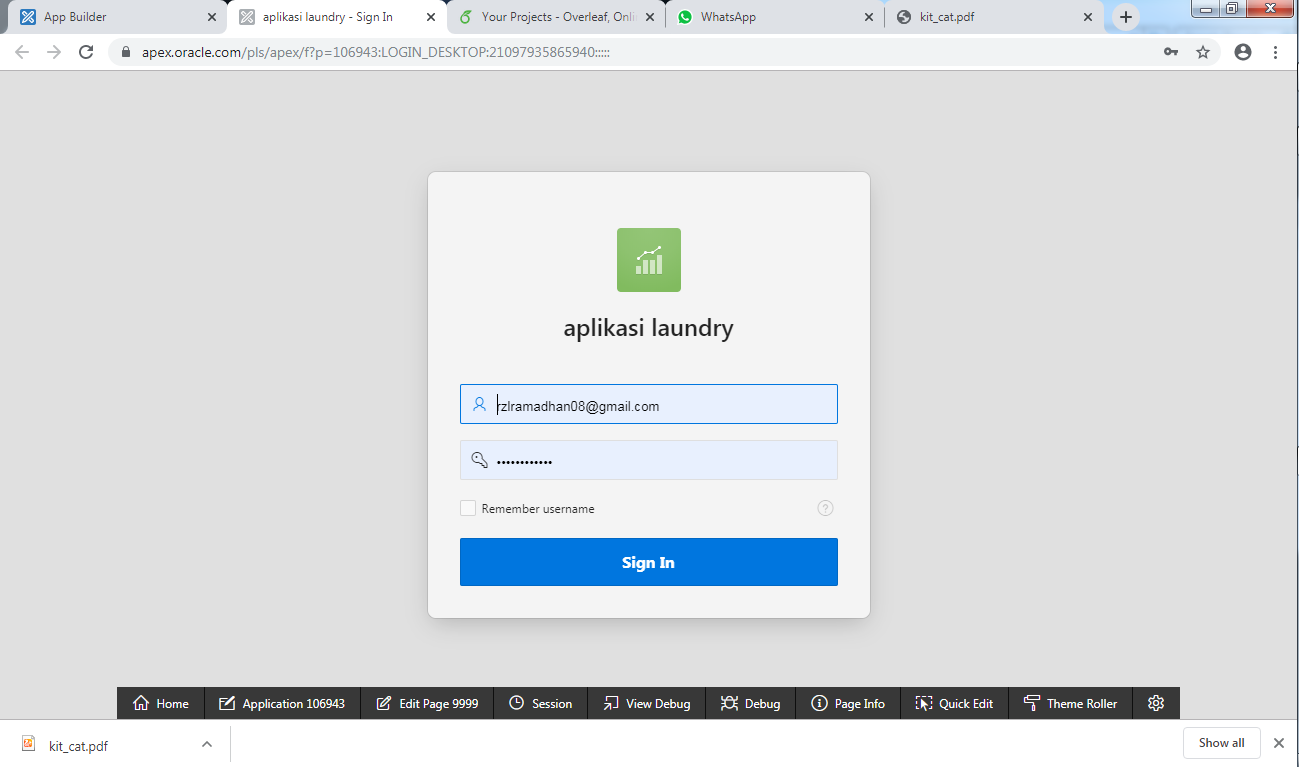
\includegraphics[scale=0.27]{gambar/Capture16.PNG}
        \caption{}
        \label{excel}
    \end{center} 
    
\item ini tampilan aplikasi saya 
    \begin{center}
         \centering
            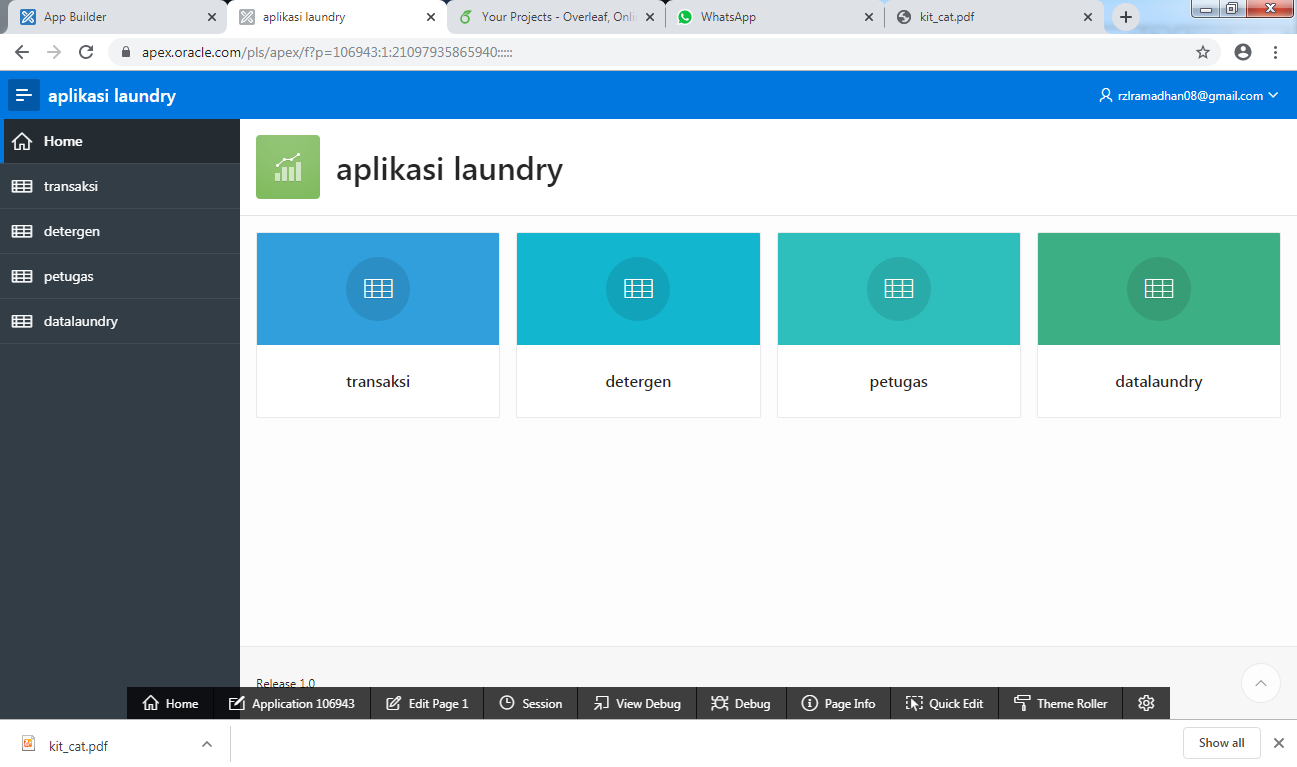
\includegraphics[scale=0.27]{gambar/Capture17.PNG}
        \caption{}
        \label{excel}
    \end{center} 
    
    \begin{center}
         \centering
            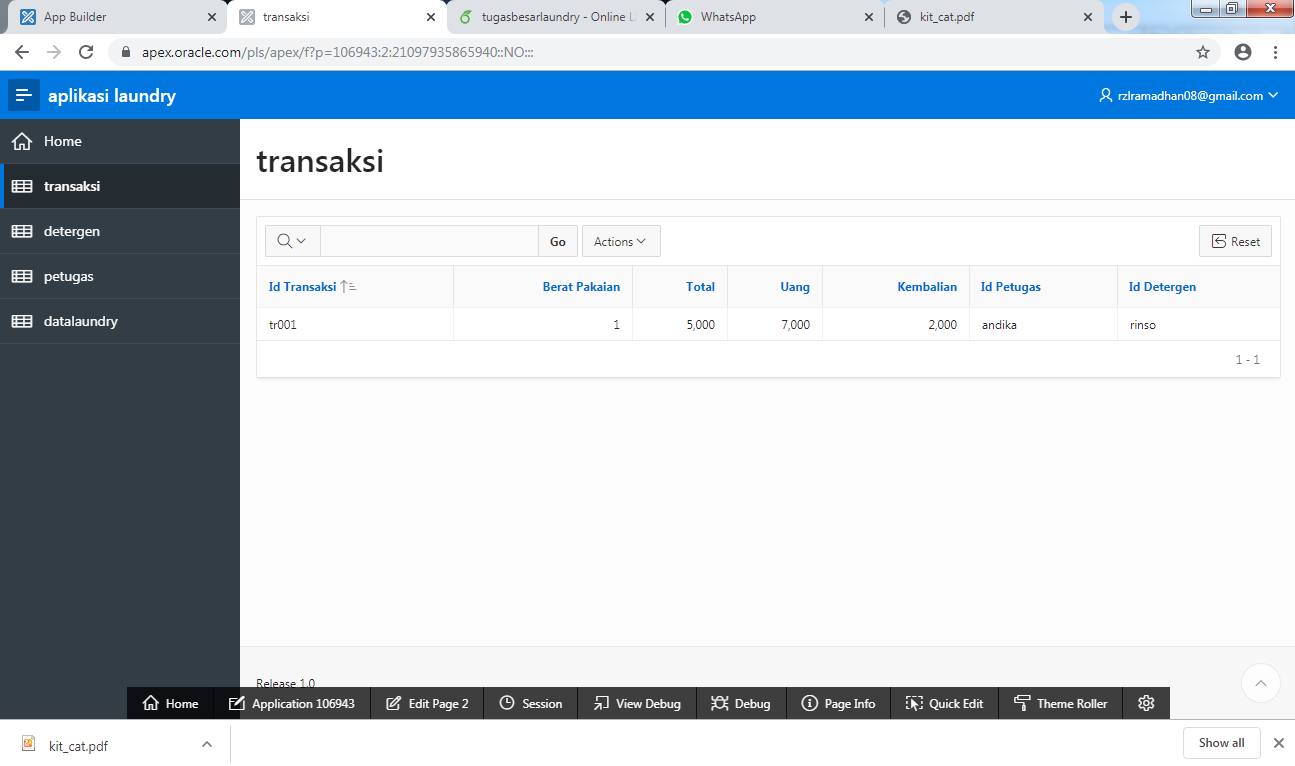
\includegraphics[scale=0.27]{gambar/Capture18.PNG}
        \caption{}
        \label{excel}
    \end{center} 
    
\end{enumerate}

\section{user dan link aplikasi}
\begin{enumerate}
\item https://apex.oracle.com/pls/apex/f?p=106943:2:21097935865940::NO:::
\item workspace:bambang
\item username:rzlramadhan08@gmail.com
\item password :081214488368
\end{enumerate}

\end{document}

